\paragraph{Histograma de gradientes orientados} ~\\
\label{subsection:hog}

	Histograma de Gradientes Orientados o HOG (por sus siglas en inglés), son descriptores de características utilizados en visión por computadora y en el procesamiento de imágenes con el objetivo de realizar detección de objetos. Fueron introducidos por N. Dalal y B. Triggs en~\cite{DT05} con el propósito de realizar detección de personas; sin embargo, su uso no se limita solamente a esa área, sino que pueden ser utilizados en otras áreas como la detección de caracteres tal y como hizo Wang et al. en \cite{wang}.
	
	Todas las imágenes, como por ejemplo la presentada en la figura~\ref{fig: Imagen Letra original}, contienen objetos locales cuyas apariencias y formas pueden ser descriptas por la distribución de los gradientes de intensidad como se puede observar en la figura~\ref{fig: Image HOG}.	Un descriptor HOG, es un vector compuesto por una combinación de histogramas que representan los gradientes de intesidad en distintas regiones de una imagen. La implementación de estos descriptores, se obtiene dividiendo a la imagen en regiones de tamaño fijo llamadas celdas como se puede observar en la figura~\ref{fig: Image HOG celdas} y posteriormente, por cada celda, se calcula un histograma de gradientes para los píxeles en la celda ~\ref{fig: Cell Histogram}. Finalmente, como se explico anteriormente, el descriptor se obtiene de combinar los histogramas obtenidos~\ref{fig: Vector HOG}. La precisión se puede incrementar si se normalizan los histogramas, es decir, si se calcula una medida de la intensidad en una región más grande de la imagen, denominada bloque y se utiliza dicho valor para normalizar las celdas contenidas en el bloque.
	
	%El descriptor HOG mantiene una cuantas ventajas con respecto a otros métodos descriptores. Dado que el descriptor HOG opera en celdas localizadas, el método mantiene la invarianza a transformaciones geométricas y fotométricas, excepto para la orientación de objetos. Dichos cambios sólo aparecerían en regiones espaciales grandes~\cite{DT05}.
	
	En el área de visión por computadora, los descriptores HOG son considerados estado del arte o \textit{state of the art} al igual que muchos otros descriptores como \textit{SIFT}, \textit{Geometric Blur}, \textit{Shape Context}, \textit{Patch descriptor}, \textit{Maximum Response of filters} y \textit{Spin image}. Los descriptores HOG, han demostrado ser útiles en la clasificación como se puede apreciar en el trabajo de Wang et al.~\cite{wang} donde se ha entrenado el clasificador Random Ferns con estos. Incluso, se puede decir que la performance obtenida con estos descriptores en dicho trabajo supera a la mayoría de los descriptores evaluados en el trabajo de De Campos et al.~\cite{dCBV09} bajo las mismas condiciones de entrenamiento. Si bien Wang et al. usan como clasificador a Random Ferns y De Campos et al. usan en su evaluación SVM, se puede apreciar en la clasificación el impacto positivo al utilizar los descriptores HOG.
	
	La binarización de los descriptores HOG es necesaria, ya que las características binarias son fáciles de computar, son compactas, se pueden almacenar fácilmente y son fáciles de comparar. En cambio, los descriptores originales tienen alta dimensionalidad y requieren sistemas con más memoria, capacidad de almacenamiento y procesamiento. Uno de los beneficios de este enfoque en la clasificación, es que escala bien con la cantidad de categorías o clases. Muchos sistemas en tiempo real como el reconocimiento de objetos~\cite{SJC08} y en el agrupamiento de puntos clave~\cite{OFL07} han incorporado este enfoque por su utilidad.

	
	\paragraph{Binarización} ~\\

		A continuación se explicará un método para la binarización de los descriptores HOG. Para binarizar es necesario calcular un vector umbral. El umbral se calcula de la siguiente manera:
		\begin{itemize}
			\item Dado $N$ descriptores HOG de dimension $D$, se forma una matriz de tamaño $N \times D$ donde cada fila representa un vector.
			\item Se seleccionan $X$ columnas al azar de la matriz con reemplazo.
			\item Respetando el orden en que fueron seleccionadas, se aplica una función sobre cada columna (la función puede ser el calculo de la mediana, la media, bootstrap, entre otros), obteniendo de esta manera un vector nuevo $W$ de dimensión $X$ tal que cada dimensión de $W$ está compuesta por un par $(z,y)$ donde $y$ es un número talque $0 \leq y \leq D$ que representa una de las columnas elegidas de la matriz y $z$ representa el valor resultante de haber aplicado la función elegida a dicha columna. Cabe aclarar que $X$ puede ser mayor o menor a $D$ por lo cual el umbral $W$ puede tener mayor o menor dimensión al final.
		\end{itemize}
		Posteriormente dicho umbral $W$ se utiliza para binarizar los vectores originales de manera sencilla: sea $v_j$ con $j \in \{1,\dots,N\}$ uno de los $N$ vectores originales y tal que $v_j = d_1,d_2,\dots,d_D$. Luego se compara cada dimensión del umbral $W$ con la $y$-esima dimensión del vector $v_j$. Si $d_y \leq z$ se asigna 0, caso contrario 1. De esta manera binarizamos el vector $v_j$ obteniendo un nuevo vector binario de dimensión $X$.

		\begin{figure}[htbp]
			\centering
			\subfloat[Imagen original\label{fig: Imagen Letra original}]{
				\fbox{ 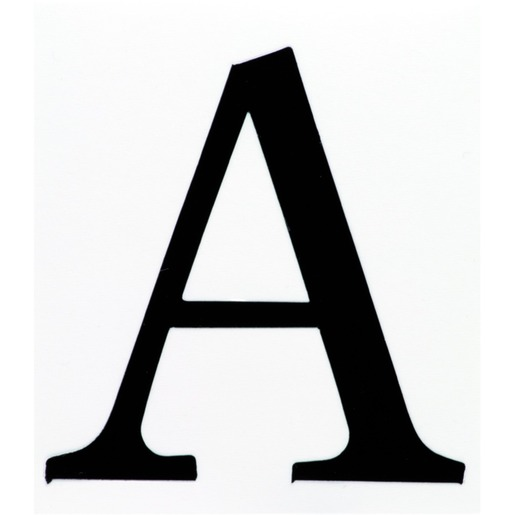
\includegraphics[scale=0.3]{img/letter_A.jpg} }
			}
			\subfloat[Descriptores HOG de la imagen original\label{fig: Image HOG}]{
				\fbox{ 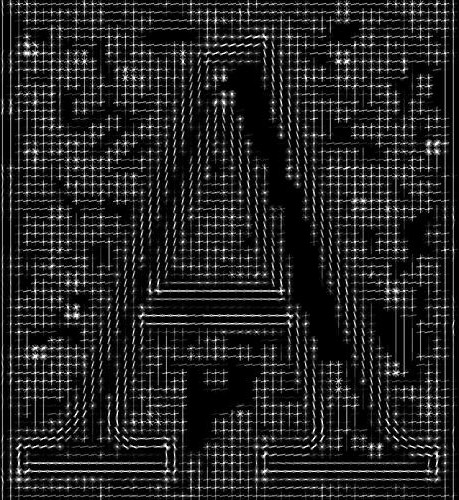
\includegraphics[scale=0.3]{img/letter_A_HOG.jpg} }
			}
			\\
			\subfloat[División por bloques de tamaño 4x4 celdas\label{fig: Image HOG celdas}]{
				\fbox{ 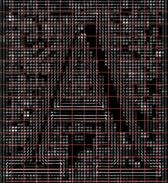
\includegraphics[scale=0.6]{img/letter_A_with_cells_2.jpg} }
			}
			\subfloat[Histograma de una celda\label{fig: Cell Histogram}]{
				\fbox{ 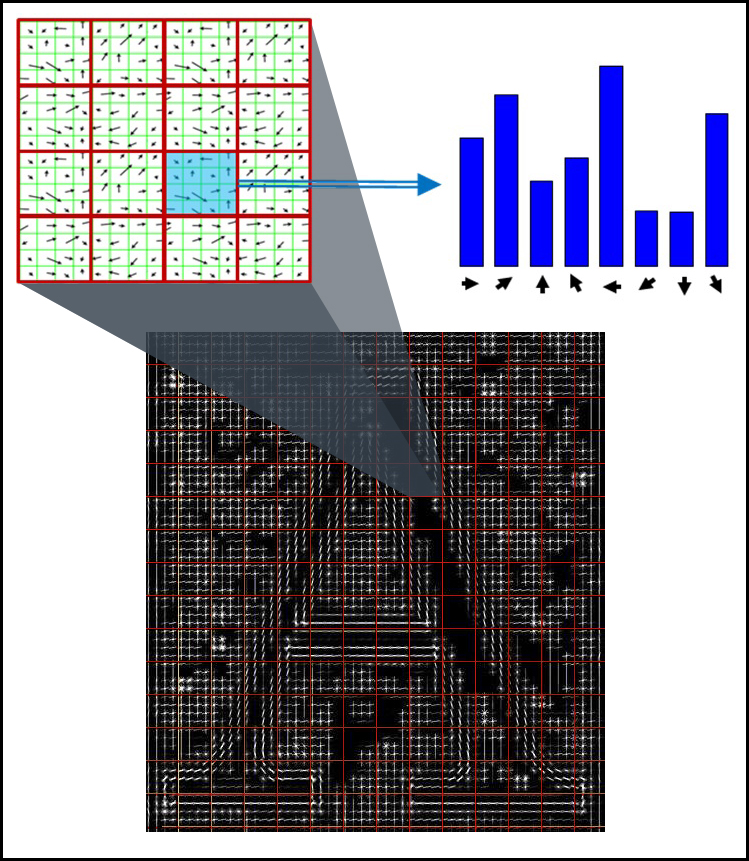
\includegraphics[scale=1.5]{img/letter_A_histogram.jpg} }
			}
			\caption{Descriptores HOG de la imagen de un caracter}
			\label{fig: HOG features}
		\end{figure}	

		\begin{figure}[htbp]
			\centering
			\fbox{ 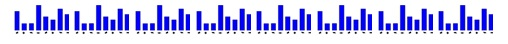
\includegraphics[scale=1]{img/feature_vector.jpg} }
			\caption[Vector HOG]{Formación del vector de características a partir de la concatenación de los histogramas. \textbf{CAMBIAR IMAGEN por algo mejor}}
			\label{fig: Vector HOG}
		\end{figure}
